\section{MobiScope Overview}
\label{sec:platform}

% This section describes the goals for our monitoring approach, and how
% \platname achieves these goals using proxying.  We show that our
% approach imposes reasonable overheads, and we describe how our
% IRB-approved study protects user privacy.

% \subsection{Goals}
% \label{sec:goals}
% Our primary goal is \emph{to monitor all the Internet traffic from
%   mobile devices regardless of the operating system, wireless access
%   technology, and the ISPs used by the mobile device}.  To achieve
% this goal, we identify the following desirable properties for a
% measurement platform:
% \begin{packedenumerate}
% \item \emph{Portable.} Our approach should work on all major device
%   OSes without requiring support from carriers or ISPs.
% \item \emph{Pervasive.} We should be able to measure traffic
%   regardless of the location, access technology, and ISPs used by
%   mobile devices.
% \item \emph{Passive.} We wish to understand the network traffic
%   naturally generated by users and their devices, requiring passive
%   monitoring.
% \item \emph{Deployable.} We want a low barrier to entry to facilitate
%   large-scale adoption with minimal impact on the user
%   experience. \tbd{We need to say easy to controlled perform
%     experiments}
% \end{packedenumerate}

In this section, we present the \platname{} plateform whose goal is
\emph{to monitor all the Internet traffic from and to mobile devices}
with the following constraints.
\begin{packedenumerate}
\item \emph{OS agnostic.} We want to monitor traffic independently of
  the OS run by the monitored device. In particular, we do not want to
  develop OS specific applications, or to root or jailbreak the phone.
\item \emph{ISP agnostic.} We want to monitor traffic without any
  support from ISPs and cellular providers.
\item \emph{Access technology agnostic.} We want to monitor traffic
  whatever the access technology used by the mobile device (Wifi, GSM,
  CDMA, UMTS, LTE, etc.)
\item \emph{Encryption agnostic.} We want to monitor traffic both in
  clear and encrypted.
\item \emph{Easy to install and setup.} We want a plateform easy to
  install, typically on a single regular desktop, and easy to setup,
  that is with no complex configuration.
\end{packedenumerate}    



\subsection{MobiScope Design}

% We now describe how we achieve these goals using proxying.
% Specifically, we use two approaches to proxy mobile traffic: secure
% proxying via virtual private networks (VPNs) and insecure transparent
% proxying.  These two approaches allow us to measure traffic with and
% without carrier interposition, respectively.

% \subsubsection{VPN Proxying}
% \label{sec:platform-vpn}

In order to monitor all Internet traffic from and to mobile devices
with the constraints we described, we designed the \platname{} plaform
on a VPN infrastructure. By instrumenting the VPN server that
mobile devices are using, we can monitor all the Internet traffic going
through the VPN tunnels. But, using a VPN infrastructure raises three
important questions. i) How ubiquitous is the VPN technology on mobile
devices?  ii) How to monitor traffic on \platname{}? iii) How to
modify traffic on \platname. We explore in the following these three key questions.

\subsubsection{VPN Technology on Mobile Devices}
\label{sec:vpn-tech-mobile-device}
The VPN technology is widely supported on the most popular mobile
OSes. Indeed, Android, BlackBerry, Bada, and iOS all support VPNs,
primarily to satisfy their enterprise clients that use VPNs to
securely connect to their enterprise networks. Also, the VPN
technology on mobile devices encapsulates all the data traffic---both
Wi-Fi and cellular. Consequently, it is possible to reach our three
first design goals: OS, ISP, and access technology agnostic.

However, to capture all Internet traffic from and to a mobile device,
a VPN must always be enabled. Currently, all iOS devices (version 3.0
and above) support a feature called \textit{VPN On-Demand}.  VPN
On-Demand forces the iOS device to use VPN tunnels when connecting to
a specified set of domains, and we configured it to be enabled for all
Internet domains. Android version 4.2 and above support an
\textit{Always On VPN} connection that is always enabled for all data
traffic, and Android version 4.0 and above provide an API that allows
applications to manage VPN tunnels. We implemented an application that
uses this API in order to provide the always on functionality for
Android 4.0 and 4.1.


% The use IPsec by mobile devices for pervasive VPN tunnels limited our
% choice of VPN daemons to manage VPN tunnels on our proxying server.
% Though VPN daemons manage tunnels created using protocols such as PPTP
% and L2TP, the ``VPN On-Demand'' feature of iOS is available only for
% VPN tunnels that use IPsec.  To the best of our knowledge, the only
% publicly available VPN daemon that uses IPsec in Linux \emph{without
%   any kernel modifications} is Strongswan~\cite{strongswan}.
% Strongswan also supports the faster IKEv2~\cite{rfc5996} based
% authentication which is supported by Android devices.

% \subsubsection{Advantages and Drawbacks of VPNs}
% \label{sec:advant-drawback-vpn}



\subsubsection{Monitoring Traffic on MobiScope}
\label{sec:monit-traff-mobiscope}




%start the discussion of the technical details. TO REWRITE
The IPsec implementation in the Linux kernel is not suitable to
traffic monitoring when the server running the VPN daemon is used to
proxy Internet traffic.  A VPN Proxy, apart from serving VPN tunnels,
relies on NAT to proxy Internet traffic.  When a mobile device
establishes a VPN tunnel, the VPN server assigns it assigned a private
IP address.  The mobile device therefore has two IP addresses, a
private address assigned by the VPN server, and a public IP address
assigned by the service provider.  The public IP address is used only
to communicate with the VPN server while all other communication uses
the private IP address.  Therefore all the traffic that would have
used the public IP address when the VPN tunnel was not present, now
uses the private IP address.  These packets that use the private IP
are encapsulated and encrypted using IPsec and sent to the VPN server.
The VPN server decapsulates these packets before forwarding them.
Before forwarding the packet, the VPN server must perform NAT because
these private IP address cannot used in the Internet.  The use of NAT
and IPsec implies that the forwarding each packet by the server is
governed by two rules: one rule to enforce IPsec encryption and
decryption of packets that contain the public IP of the mobile device,
and the other that enforces NAT for packets with the private IP
address.

\begin{figure}
\begin{center}
  \subfloat[Packet from mobile device. \emph{Tcpdump can capture
    packets at step (2)~d~$\rightarrow$~m, (4)~v~$\rightarrow$~w, and
    (7)~m~$\rightarrow$~w.}]{\label{fig:packet-monitor-a}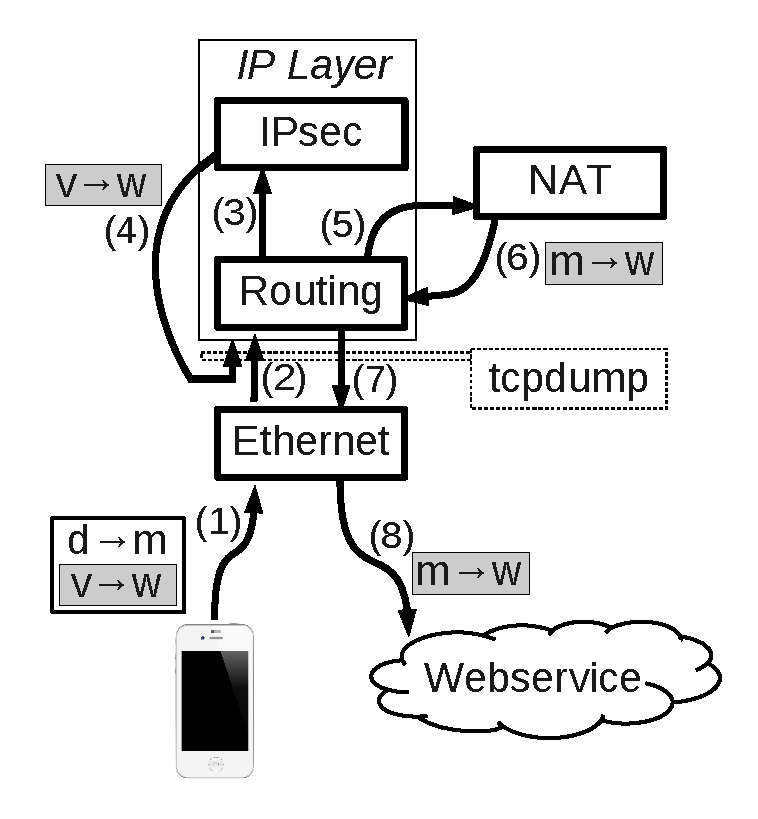
\includegraphics[width=0.47\columnwidth]{figures/packet-monitoring-a.pdf}}
  \hspace{0.05\columnwidth} \subfloat[Packet to mobile
  device. \emph{Tcpdump can capture packets at step
    (2)~w~$\rightarrow$~m and (7)~m~$\rightarrow$~d, however it is
    cannot log the packet
    w~$\rightarrow$~v.}]{\label{fig:packet-monitor-b}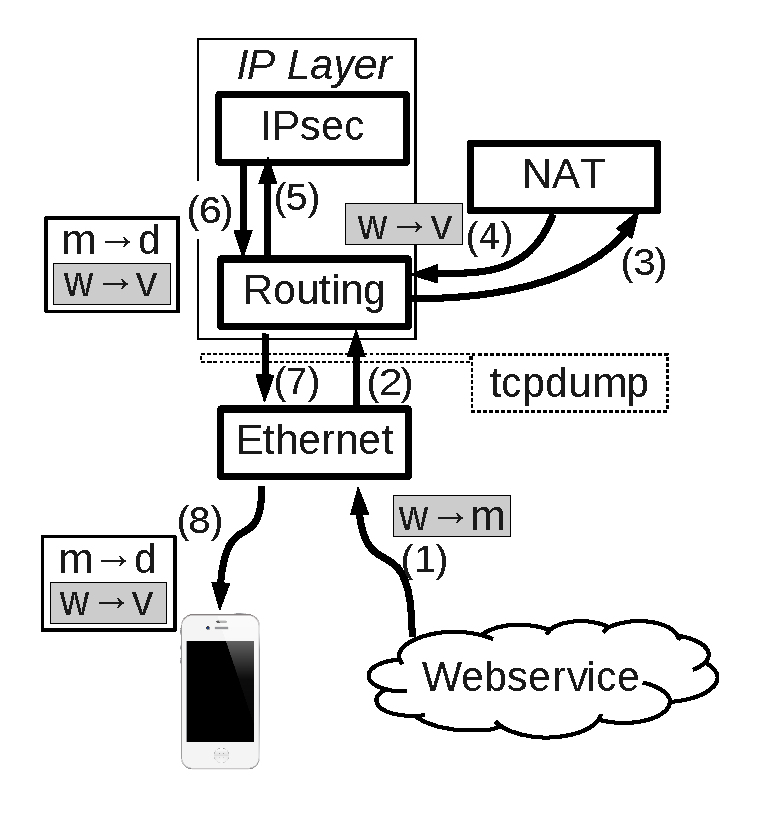
\includegraphics[width=0.47\columnwidth]{figures/packet-monitoring-b.pdf}}
  \newline \subfloat[Packet from mobile device. \emph{Tcpdump
    monitoring packets on the tun device can capture packets at step
    (5)~v~$\rightarrow$~w, and
    (6)~v'~$\rightarrow$~w.}]{\label{fig:packet-monitor-c}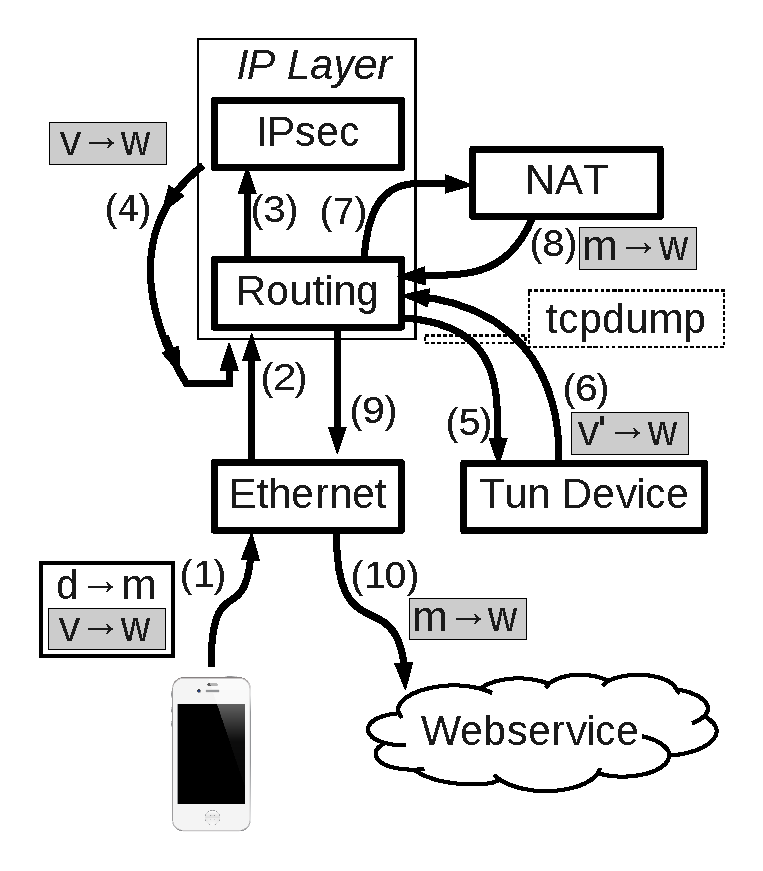
\includegraphics[width=0.47\columnwidth]{figures/packet-monitoring-c.pdf}}
  \hspace{0.05\columnwidth} \subfloat[Packet to mobile
  device. \emph{Tcpdump monitoring packets on the tun device can
    capture packets at step (5)~w~$\rightarrow$~v', and
    (6)~w~$\rightarrow$~v.}]{\label{fig:packet-monitor-d}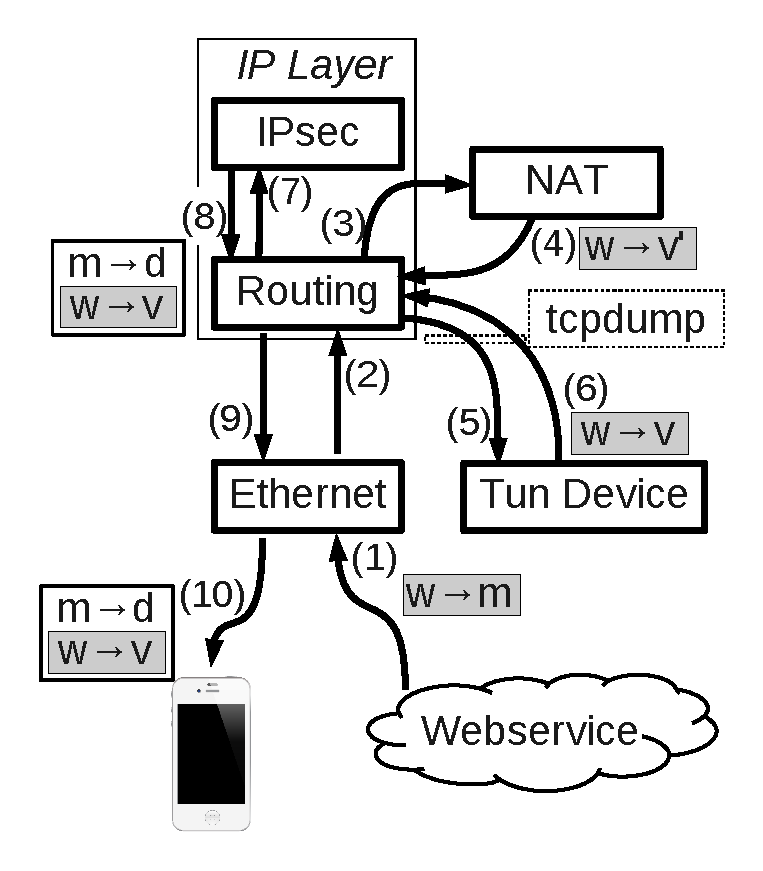
\includegraphics[width=0.47\columnwidth]{figures/packet-monitoring-d.pdf}}
  \newline
\begin{small}
\begin{tabular}{|c|p{0.8\columnwidth}|}
\hline
Symbol & Description \tabularnewline
\hline
d & IP address of the mobile device assigned by its ISP. \tabularnewline
m & IP address of the \platname server. \tabularnewline
w & IP address of the server providing the Webservice. \tabularnewline
(i) & The i-th step of packet processing. \tabularnewline
\fbox{a $\rightarrow$ b} & Packet with source IP \emph{a} and destination IP \emph{b}. \tabularnewline
v & IP address of the mobile device in the VPN tunnel. \tabularnewline
v' & IP address of the mobile device while looping through tun device. \tabularnewline

\hline
\end{tabular}
\end{small}
\end{center}
\caption{Packet monitoring in the VPN proxy.}
\label{fig:packet-monitoring}
\end{figure}


\begin{figure}
\begin{center}
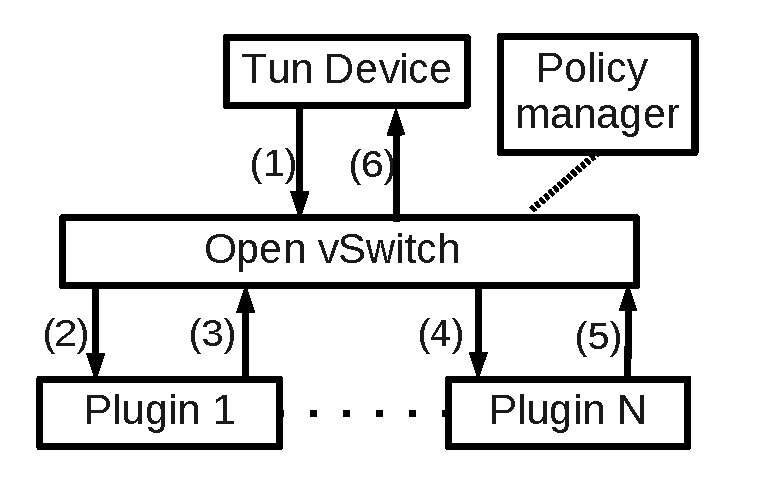
\includegraphics[width=0.8\columnwidth]{figures/packet-monitoring-plugin.pdf}
\end{center}
\caption{Plugin Infrastructure on \platname.}
\label{fig:packet-monitoring-solution}
\end{figure}


An association between the mobile device and a packet is possible only
if the packet encapsulated within an IPsec packets is monitored in the
clear.  However, the current implementation of NAT and IPsec makes
this association of packets with the mobile devices non-trival.  A
packet from the mobile device, encrypted using IPsec, needs to be
decrypted before undergoing NAT.  As shown in
\fref{fig:packet-monitoring-problem}, because the IPsec computations
take place after the NAT computations, the kernel loops the packet
back to the IP layer after decryption.  This looping allows the packet
monitor to observe the IPsec packet before and after
decryption\footnote{A similar operation takes place if the mobile
  devices communicate with each other over P2P however we do not
  discuss this scenario due to lack of space.}.  When multiple flows
pass through the VPN server, the packet monitor can use the private IP
address to associate the packets with the mobile device.  Once the NAT
operation is performed the packet is forwarded via the network card.
When the network card receives a packet intended for the mobile
device, as shown in \fref{fig:packet-monitoring-problem}, the packet
first undergoes NAT followed by IPsec encryption.  The encrypted
packet is then sent to the mobile device.  Because the packet is not
looped through the packet monitor before encryption, the packet
monitor is not able to see the packet after NAT and before encrpytion.
This implies without any modifications, any off the shelf packet
monitor shall fail to associate the packets destined for mobile
devices with the corresponding mobile device.

\subsubsection{Modifying Traffic on MobiScope}
\label{sec:modif-traffic-mobiscope}



% \begin{figure}
% \begin{center}
% \includegraphics[width=0.8\columnwidth]{figures/tun-device.pdf}
% \end{center}
% \caption{Tun-tap device to loop packets for packet monitoring.}
% \label{fig:packet-monitoring-solution}
% \end{figure}

% To monitor the packets that are encapsulated within IPsec packets we
% route the packets through a tun-tap device before encryption and after
% decryption.  As shown in \fref{fig:packet-monitoring-solution},

% \subsubsection{Transparent Proxy}
% \label{sec:platform-transparent-proxy}


\subsection{Feasibility}


\subsection{Limitation}
\platname {} has reached all the design goals, making this platform an
excellent choice to monitor traffic for mobile devices. However,
\platname{} has one limitation: because all the traffic between mobile
devices and \platname{} is encrypted, we cannot observe any traffic
modification made by ISPs. Indeed, ISPs that modify traffic (e.g., to insert
advertisements \tbd{AR: give a reference}) must perform deep packet
inspection, which is not possible when the traffic is encrypted.  In
this section, we assess to which extent this issue is a practical
limitation for \platname.


\tbd{AL: put tripwire experiments here to show that ISP traffic
  modification does not impact much Mobiscope. }

%%% Local Variables: 
%%% mode: latex
%%% TeX-master: "main.tex"
%%% End: 
